% ****** Start of file apssamp.tex ******
%
%   This file is part of the APS files in the REVTeX 4.1 distribution.
%   Version 4.1r of REVTeX, August 2010
%
%   Copyright (c) 2009, 2010 The American Physical Society.
%
%   See the REVTeX 4 README file for restrictions and more information.
%
% TeX'ing this file requires that you have AMS-LaTeX 2.0 installed
% as well as the rest of the prerequisites for REVTeX 4.1
%
% See the REVTeX 4 README file
% It also requires running BibTeX. The commands are as follows:
%
%  1)  latex apssamp.tex
%  2)  bibtex apssamp
%  3)  latex apssamp.tex
%  4)  latex apssamp.tex
%
\documentclass[%
 reprint,
%superscriptaddress,
%groupedaddress,
%unsortedaddress,
%runinaddress,
%frontmatterverbose,
%preprint,
%showpacs,preprintnumbers,
%nofootinbib,
%nobibnotes,
%bibnotes,
 amsmath,amssymb,
 aps,
%pra,
%prb,
%rmp,
%prstab,
%prstper,
%floatfix,
]{revtex4-1}

\usepackage{graphicx}% Include figure files
\usepackage{dcolumn}% Align table columns on decimal point
\usepackage{bm}% bold math
%\usepackage{hyperref}% add hypertext capabilities
%\usepackage[mathlines]{lineno}% Enable numbering of text and display math
%\linenumbers\relax % Commence numbering lines
\usepackage{mathrsfs}
\usepackage{float}
%\usepackage[showframe,%Uncomment any one of the following lines to test
%%scale=0.7, marginratio={1:1, 2:3}, ignoreall,% default settings
%%text={7in,10in},centering,
%%margin=1.5in,
%%total={6.5in,8.75in}, top=1.2in, left=0.9in, includefoot,
%%height=10in,a5paper,hmargin={3cm,0.8in},
%]{geometry}
\usepackage[spanish]{babel}
\selectlanguage{spanish}
\usepackage[utf8]{inputenc}
\usepackage{esint}
\begin{document}

%\preprint{APS/123-QED}

\title{Sistemas dinámicos}% Force line breaks with \\


\maketitle

% ████████ ███████ ██████  ███    ███  ██████
%    ██    ██      ██   ██ ████  ████ ██    ██
%    ██    █████   ██████  ██ ████ ██ ██    ██
%    ██    ██      ██   ██ ██  ██  ██ ██    ██
%    ██    ███████ ██   ██ ██      ██  ██████

\section{Introducción}

\textbf{\# Función de Lipschitz: }
$\mathrm{Una}$ función ${f}: \mathrm{M} \rightarrow \mathrm{N},$ entre dos espacios métricos con métricas $d_{M} d_{N}$ satisface la condición de Lipschitz(o es Lipschitz continua) si existe una constante $K>0$ tal que:
$$
d_{N}(f(x), f(y)) \leq K d_{M}(x, y) \quad \forall x, y \in M
$$


$K$ es la constante Lipschitz de la función.
Si $M$ es $\mathbb{R}^{m}$ y $N$ es $\mathbb{R}^{n}$


$$
\|f(x)-f(y)\| \leq K\|x-y\| \quad \forall x, y \in \mathbb{R}^{m}
$$

$\sim$ Toda función Lipschitz continua es uniformemente continua y por tanto continua.

$\sim$ Continuidad $\Rightarrow \exists$ soluciones (Teorema Peano, valido para EDO) 

% El teorema de Picard-Lindelöf (o Cauchy-Lipschitz) establece bajo qué condiciones puede asegurarse la existencia y unicidad de la solución de una ecuación diferencial ordinaria dado un problema de Cauchy.
$>$ \textbf{Teorema de Picard-Lindelöf}:  Sea $f(t, x): \Omega \subseteq R \times R^{n} \rightarrow R^{n}$ con $\Omega$ un abierto, una función continua y localmente Lipschitz respecto de $x$. Entonces, dado $\left(t_{0}, x_{0}\right) \in \Omega$ es posible hallar un intervalo cerrado $\mathrm{I}_{\alpha}=\left[\mathrm{t}_{0}-\alpha, \mathrm{t}_{0}+\alpha\right] \in \mathbb{R}, \mathrm{a}>0$ donde existe una
solución de problema de Cauchy
$$
\left\{\begin{array}{l}
x^{\prime}=f(t, x) \\
x\left(t_{0}\right)=x_{0}
\end{array}\right.
$$
que cumple que los pares $(t, x(t)) \in \Omega,$ para todo $t$ en $I_{\alpha}$ y esa solución es única



\textbf{\#} \textbf{Punto Fijo}(equilibrio, estado estacionario, punto singular): Punto del espacio de fases que no evoluciona en el tiempo.

$>>$ Encontrar puntos fijos($x^*$):
\begin{itemize}
  \item Caso continuo: Por ser $\frac{dx}{dt}=f(x)$ resolver, $f(x^*) = 0$.
  \item Caso discreto: Resolver, $x^* = f(x^*)$
\end{itemize}

\textbf{\# Atractor:} Conjunto hacia el cual un sistema dinámico evoluciona con el tiempo. Puede ser un punto, una curva o una estructura más complicada.

\textbf{\# Punto fijo estable:} para todos los valores iniciales $x 0$ cerca de $x^{*}$ el sistema converge a $x^{*}$ cuando $t \rightarrow \infty .$

\textbf{\# Punto fijo marginalmente estable (neutral)}: para todos los valores iniciales $x_0$ cerca de $x^{*},$ el sistema permanece cerca de $x^{*}$ pero no converge a $x^{*}$.

\textbf{\# punto fijo inestable}: para valores iniciales $x_0$ muy cerca de $x^{*},$ el sistema se aleja de $x^{*}$

\textbf{\# Autonomía}

$$\underbrace{\frac{d x}{d t}=\dot{x}=f(x, \lambda, t) }_{\textbf{No autónomo}}
,\quad 
\underbrace{\frac{d x}{d t}=f(x, \lambda)}_{\textbf{Autónomo}}
$$

\textbf{\# Estabilidad de Lyapunov(Lineal)(Liapunov en algunos libros):} Un punto de equilibrio del sistema $\mathrm{x}^{\prime}(\mathrm{t})=\mathrm{Ax}(\mathrm{t})$ es estable en el sentido de Lyapunov (ESL) si para cualquier $\varepsilon>0$ existe un valor $\delta\left(t_{0}, \varepsilon\right)>0$ tal que:
$$
\left\|x\left(t_{0}\right)-x^{*}\right\|<\delta \Rightarrow\left\|x(t)-x^{*}\right\|<\varepsilon
$$
independiente de $t$. Si ademàs $\delta$ no depende del tiempo inicial $t_{0}$ el punto es uniformemente estable

$\sim$ En criollo: "Si arranco \textit{cerca} del equilibrio, la evolución temporal ocurre \textit{cerca} del equilibrio", \textit{cerca} hace referencia a una cantidad finita, como en topología en algunos casos, los epsilon y delta se pueden hacer arbitrariamente chicos.

$\sim$ Segun el tamaño de $\delta(t_0, \varepsilon)$, tendre estabilidad local($\delta$ chico) o global($\delta$ grande).

$\sim$ Para sistemas lineales todos los puntos de equilibrio son globales, o son puntos aislados o son subespacios invariantes (Las trayectorias que empiezan en un dado subespacio evolucionan dentro de ese subespacio).

$\sim$ Sistemas no lineales: Hay estabilidad asintótica y de lyapunov.


\textbf{\# Estabilidad Asintótica:} Es (ESL) y además se cumple $\left\|x(t)-x^{*}\right\| \rightarrow 0$ cuando $t \rightarrow \infty$ el punto es asintóticamente estable

\textbf{$\cdot$ Estabilidad orbital (2D en adelante)}

\textbf{\# Órbita estable} $x(t)$ es una órbita estable si dado $\epsilon>0,$ existe $\delta(\epsilon)>0$ tal que para cualquier otra solución $y(t),$ tal que $\| x\left(t_{0}\right)-y\left(t_{0}\right) \|<\delta \Rightarrow \| x(t)-y(t) \| < \delta$ para todo $t>t_{0}$

\textbf{\# Órbita asintóticamente estable} $x(t)$ es una órbita asint. estable si es estable $y$ además para cualquier otra solución $y(t),$ existe $\delta$ tal que $\| x\left(t_{0}\right)-y\left(t_{0}\right) \|<\delta$ entonces $\lim _{t \rightarrow \infty} \| x\left(t\right)-y\left(t\right) \| =0$


$>$ \textbf{Analisis lineal:}
$
\left\lbrace 
\begin{array}{l}
\dot{x}=f(x) \\
f\left(x^{*}\right)=0
\end{array}
\right.
$

Para analizar estabilidad de $x^{*}$, introduzco una perturbación

$
\begin{array}{c}
x = x^{*}+\varepsilon, \quad \varepsilon<<1 \\
\dot{x}=\dot{x}^{*}+\dot{\varepsilon}=0+\dot{\varepsilon}=f\left(x^{*}+\varepsilon\right)=f\left(x^{*}\right)+\varepsilon f_{x}\left(x^{*}\right)+O\left(\varepsilon^{2}\right) \\
\dot{\varepsilon} \approx \varepsilon f_{x}\left(x^{*}\right)=\lambda \varepsilon \quad \lambda \equiv f_{x}\left(x^{*}\right)
\end{array}
$

Es decir, tenemos ahora una ecuación diferencial lineal para el comportamiento de la perturbación y cuya solución es

\begin{itemize}\centering
  \item[]  $\varepsilon(t)=A \mathrm{e}^{\lambda t}$
\end{itemize}

Entonces:

$$
\begin{aligned}
\frac{d x}{d t}=f(x, r), & \qquad f\left(x^{*}, r\right)=0 \\
\frac{d f\left(x^{*}, r\right)}{d x} &=\left\{\begin{array}{ll}
<0 & \text { Estable } \\
>0 & \text { Inestable }
\end{array}\right.
\end{aligned}
$$

Ya que la perturbación decrece o crece respectivamente. Si $\lambda=0$ no podemos decir nada.



\begin{figure}[ht!]
  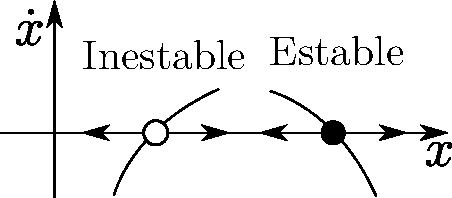
\includegraphics[width = 0.28\textwidth]{estable-Inestable.pdf}
  \caption{\label{fig:figura1} Criterio de estabilidad.}
\end{figure}

\section{Bifurcaciones}

\subsection{Bifurcaciones 1D}

La estructura cualitativa del flujo puede cambiar cuando cambian los parámetros. Los puntos fijos pueden crearse o destruirse, o su estabilidad puede cambiar.

Estos cambios cualitativos de la dinámica se llaman bifurcaciones, y los valores de los parámetros para los cuales se producen se llaman puntos de bifurcación. 

En sistemas de 1D hay 3 bifurcaciones fundamentales que se asocian a la creación y destrucción de equilibrios o cambios de estabilidad.

% $$
% (\exists K > 0: 
% d_{N}(f(x), f(y)) \leq K d_{M}(x, y), \forall x, y \in M)
% \Leftrightarrow f es de Lipschitz
% $$





\section{Mapeos 1D}

\# \textbf{Definición: } $
x_{k+1} = f(x_k , r)
$

$>$ \textbf{Analisis lineal:}
$
\left\lbrace 
\begin{array}{l}
x_{k+1} = f(x_k , r) \\
x^{*} = f(x^{*}, r)
\end{array}
\right.
$

Para analizar estabilidad de $x^{*}$, introduzco una perturbación

$x_k = x^{*}+\varepsilon_k, \quad \varepsilon_k <<1 $

$\ x_{k+1} = {x}^{*} + \varepsilon_{k+1}$

$\ x_{k+1} = f\left(x^{*}+\varepsilon_{k}, r \right) 
= f\left(x^{*}, r\right)
+ \varepsilon_{k} f_{x}\left(x^{*}, r\right)
+ O\left(\varepsilon^{2}_{k}\right)$

$\varepsilon_{k+1} \approx \varepsilon_{k} f_{x}\left(x^{*}, r\right)
= \lambda^n \varepsilon_0, \quad \lambda := f_{x}\left(x^{*},r\right)$

Modulo de perturbación crece si $|f_{x}\left(x^{*},r\right)| = |\lambda| > 1$

Entonces:

$$
\begin{aligned}
|f_{x}\left(x^{*},r\right)| = |\lambda| &=\left\{\begin{array}{ll}
<1 & \text { Estable } \\
>1 & \text { Inestable } \\
=1 & \text { Marginalmente estable } \\
=0 & \text { Superestable }
\end{array}\right.
\end{aligned}
$$

\# \textbf{Orbita periódica:} De período $p$ si es el mínimo numero tal que: $
x_0 = f(x_{p-1},r)
$

$>$ Orbita de periodo p $\Rightarrow$ p puntos fijos de $f^p$ 

$\quad x_{k+p} = f^p(x_{k},r) = x_{k}$ 

$>$ Los $\lambda$ de los p puntos fijos:

$\quad | (f^p)'(x_k, r) | < 1, \forall 0 \leq k \leq p-1$

$>$ Alcanza con analizar un solo punto fijo

$\quad (f^p)'(x_0, r) =
(f^p)'(x_1, r) =
... =
(f^p)'(x_{p-1}, r)$

$>$ La derivada :

$\quad (f^p)'(x_k, r) = 
\prod_{k=0}^{p-1} 
|f ' (x_k, r)|
$

\section{Matematica de sistemas biologicos}

\textbf{$>$ Modelo de Malthus(Crecimiento exponencial):}

$$\frac{d x}{d t}=r x, \quad 
r=\eta-\mu = \text{natalidad - mortalidad}$$


\textbf{$\cdot$ Catastrofe malthusiana:} La población crece mas rápido que la capacidad de producir alimento.

$$\frac{dh}{dt} = rh, \quad \frac{da}{dt} = k$$

$$c(t)=\frac{a(t)}{h(t)}=\frac{a_{0} k t}{h_{0} e^{r t}}=c_{0} k t e^{-r t} \longrightarrow c_{\text {crit }} \rightarrow t_{\text {crit }}$$

$$
\frac{c_{\text {crit }}}{c_{0}}=k t_{\text {crit }} e^{-r t_{\text {cint }}} \rightarrow t_{\text {crit }}=-W\left(-r \frac{c_{\text {crit }}}{c_{0}} e^{-r / k}\right) ^\text {Función de} _\text {Lambert}
$$

Funcion de Lambert:

$$W=f^{-1}(z),\quad $$

$$
\begin{array}{l}
\frac{d x}{d t}=r x\left(1-\frac{x}{K}\right) \\
\frac{d x}{d t}=0 \Rightarrow\left\{\begin{array}{l}
x=0 \\
x=K
\end{array}\right. \\
\frac{d f}{d x}=r\left(1-2 \frac{x}{K}\right)
\end{array}
$$

\textbf{$\cdot$ Mapeo Beverton Holt(Crecimiento limitado):}

En 1957 Beverton y Holt propusieron un mapeo que reproducia el comportamiento de ecuación logística

\text{Mapeo logístico: }

$$
% \text{Mapeo logístico: }
x_{n+1}=\frac{r x_{n}}{1+\frac{r-1}{K} x_{n}}$$


$
\text{Puntos fijos:}
\left\{
\begin{array}{ll}
  x=0 & \text { Estable si } 0<r<1 \\ 
  x=K & \text { Estable si } r<1
\end{array}
\right.$ 


La solución es $x_{n}=\frac{K x_{0}}{x_{0}+\left(K-x_{0}\right) r^{-n}}-\rightarrow K$

Para hallarla se hace el cambio de variable:
$
u_{n}=1 / x_{n}
$

$$
\frac{1}{u_{n+1}}=\frac{1}{u_{n}} \frac{K r}{K+\frac{r-1}{u_{n}}} \longrightarrow u_{n+1}=\frac{K u_{n}+r-1}{K r}=\frac{1}{r}\left(u_{n}+\frac{r-1}{K}\right)
$$

\textbf{$\cdot$ Logística con delay }

$$
\begin{aligned}\centering
% &\text { Logística con delay }\\
&\begin{array}{l}
\frac{d N}{d t}=f(N(t), N(t-T)) \quad T>0 \\
\frac{d N}{d t}=r N(t)\left[1-\frac{1}{K} \int_{-\infty}^{t} u(t-s) N(s) d s\right] \\
\begin{aligned}
u(t-s)=\delta(t-T-s) \Rightarrow \int_{-\infty}^{t} u(t-s) N(s) d s=N(t-T)
\end{aligned} \\
\frac{d N}{d t}=r N(t)\left[1-\frac{N(t-T)}{K}\right]
\end{array}
\end{aligned}
$$

\textbf{$\cdot$ Poblaciones estables Lotka:}


\begin{itemize}
  \item[] $\nu(t)$ Natalidad
  \item[] $\rho(\tau)$ Probabilidad de supervivencia hasta la edad $\mathrm{T}$
  \item[] $\phi(\tau)$ Fertilidad a la edad $\mathrm{T}$
  \item[] $\int_{0}^{\infty} \rho(\tau) d \tau$ Esperanza de vida
\end{itemize}


Por otro lado, podemos calcular la tasa de natalidad $v(t)$ en un tiempo dado a partir de la composición de la población, para eso debemos tener en cuenta la historia previa:
$v(t)=\int_{0} v(t-\tau) \rho(\tau) \phi(\tau) d \tau$
Es decir, debemos contar la cantidad de mujeres que nacieron en $\mathrm{t}-\mathrm{T}$ que sobrevivieron hasta t y considerar como contribuyen a la tasa de natalidad total dada su edad.


$v(t)=\int_{0}^{\infty} v(t-\tau) \rho(\tau) \phi(\tau) d \tau \quad$ Natalidad
Propongo una solución exponencial para la ecuación anterior $v(t)=v(0) e^{r t}$
con $\mathrm{r}$ desconocidp
Reemplazo y obtengo
$v(t)=\int_{0}^{\infty} v(t) e^{-r \tau} \rho(\tau) \phi(\tau) d \tau \Rightarrow 1=\int_{0}^{\infty} e^{-r \tau} \rho(\tau) \phi(\tau) d \tau$
La ecuación de la derecha se conoce como ecuación de Lotka. La integral es siempre positiva y decrece monotonamente con $\mathrm{r}$. por eso hay un solo valor de $\mathrm{r}$ que satisface la ecuación, $\mathrm{r}_{1}$

Poblaciones estables - Lotka
Obtenido el valor de r, puedo calcular la población total a un tiempo dado
$N(t)=\int_{0}^{\infty} v(t-\tau) \rho(\tau) d \tau=\int_{0}^{\infty} e^{r_{1}(\tau-\tau)} \rho(\tau) d \tau$
Si quiero saber que cantidad de mujeres de una dada edad han sobrevivido hasta tiempo t calculo
$$
\frac{v(t-\eta) \rho(\eta)}{N(t)}=\frac{v_{0} e^{r_{1}(\tau-\eta)} \rho(\eta)}{\int_{0}^{\infty} v_{0} e^{r_{1}(\tau-\tau)} \rho(\tau) d \tau}-\stackrel{t \rightarrow \infty}{\rightarrow} \int_{0}^{\infty} e^{-r_{1} \tau} \rho(\tau) d \tau
$$
EI 'límite es una constante y es la estructura etaria buscada por Lotka

\textbf{$\cdot$ Poblaciones estables - Matrices de Leslie:}


Leslie al igual que Lotka, buscaba hallar la forma de un perfil estacionario, pero en modelo discreto. Introdujo un modelo para el crecimiento del número de hembras en una población no sujeta a procesos migratorios ni a limitaciones que pueda imponer el ambiente. La población está estratificada en edades y a lo largo del tiempo los individuos pueden permanecer en el mismo estrato etario durante un tiempo y finalmente moverse al nivel siguiente. Consideremos un caso con dos niveles etarios
$$
N_{1}(t+1)=f_{1} N_{1}(t)+f_{2} N_{2}(t)
$$
$N_{2}(t+1)=s_{1} N_{1}(t)$
Donde $f$, es la fecundidad de las hembras cada grupo etario y representa el valor media del número de descendientes per cápita de hembras de edad Por otro lado debemos evaluar la supervivencia de las hembras, que caracterizamos mediante una tasa media de supervivencia por edad $s$.

\section{Ejercicio 2}

$>$ \textbf{Analisis lineal 2D:}

\begin{figure*}[ht!]
  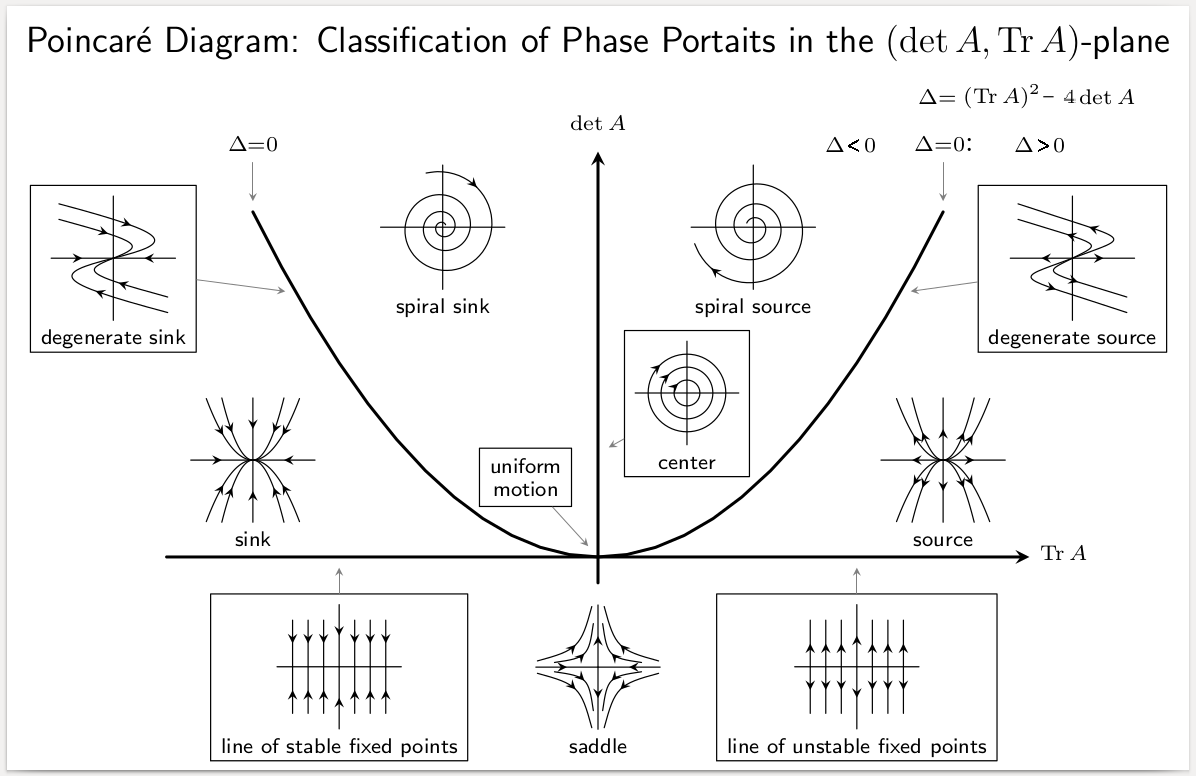
\includegraphics[width = 0.98\textwidth]{Stability_Diagram.png}
  \caption{\label{fig:figura1} Criterio de estabilidad.}
\end{figure*} 

\end{document}
%
% ****** End of file apssamp.tex ******
